% !TEX root = ../main.tex

\section{introduction}
\label{sec:org662677c}

As neural network models are able to learn increasingly more abstract representations via deeper networks, representation learning and self-supervision~\citep[see, e.g.,][]{XX,YYY,ZZZ}, it is reasonable to expect that they also get better at predicting more abstract labels. 
Beyond identifying object types~\mdr{REF}, performing face recognition~\mdr{REF}, \mdr{doing what with} expressions~\mdr{REF}, neural networks should soon be able to predict genres/categories of text, image and sound at high levels of accuracy. 
Towards this goal, there is a significant volume of recent work on building neural networks with high-level of understanding in the embedding space~\mdr{REF}.
However, there seems to be limited research on developing loss functions that are adapted for these higher level concepts in the output space.

\mdr{Briefly and concretely describe the abstract labeling task that we are interested in.}

To situate the specific problem that we tackle in this paper, it is helpful to consider Figure~\ref{fig:tree} so as to disambiguate our terminology. 
Figure~\ref{fig:tree} shows \mdr{what}.
There seems to exist a consensus over the terms \emph{multiclass} and \emph{multilabel learning}, meaning mutually exclusive and mutually inclusive labels, respectively \todo{source}. 
Multilabel learning can therefore be seen as a subdomain of multiclass learning, where more than one class can be true for the same example. 
Within multilabel training, we introduce the distinction between multi-instance multilabel~\citep[e.g.,][]{multiInstance}) and uni-instance multilabel. 
\mdr{vague: Multi-instance multilabel classification refers to tasks where elements within each example can be singled-out and assigned one or more labels; examples include objects \mdr{not a task} in an image or tokens in a text.}
Uni-stance multilabel classification is \mdr{define it}.
\begin{itemize}
\item \mdr{Now explain that the task introduced in the second paragraph is an instance of uni-instance multilabel classification.}
\item \mdr{Now make the distinction between fixed label counts and varying label counts}
\item \mdr{Little work has been done on the uni-instance, ML MC prediction with a varying number of classes}
\item \mdr{Identify the shortcomings o prior work on the task that we care about}
\end{itemize}

\begin{figure}[t]
\centering
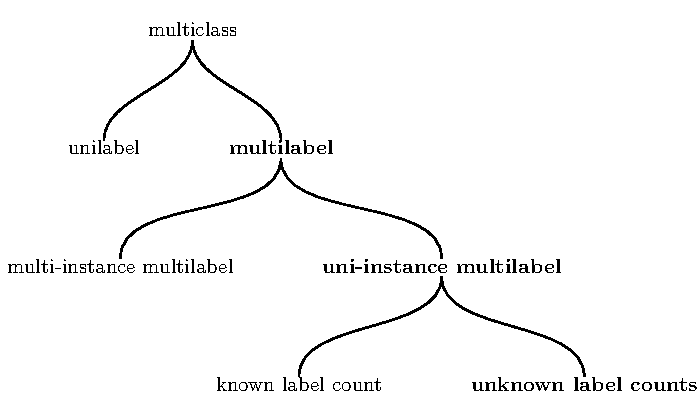
\includegraphics[width=.9\linewidth]{./tree/Tree.pdf}
\caption{\label{fig:tree}
Clarifying ``multiclass'' classification problems.
In this paper we focus on the uni-instance, multilabel, multiclass classification problem with a varying number of labels (the bottom right hand side of the tree).
\mdr{Image source ...}}
\end{figure}

\mdr{Now we have a paragraph in which you clearly describe your proposed line of attack}

\mdr{Now we have a paragraph that explains the results that we have obtained with our proposed approach}

\mdr{Now we have a paragraph with our main contributions:}
\begin{itemize}[leftmargin=*]
\item \mdr{Contribution 1}
\item \mdr{Contribution 2}
\item \mdr{Contribution 3}
\end{itemize}

\mdr{The remainder of the paper is organized as follows. Expand.}

\vspace*{3cm}
\mdr{Move all of the content to other sections, e.g., to background section or to related work. Also, try to avoid the meandering narrative that touches on many points but sometimes forgets to make explicit what its main point is.}

In this paper we focus on uni-instance multilabel training (sparse occurences of the term holistic can be found in the literature to describe this phenomenon for image \cite{holisticImageDescriptors,holisticLungs} and a recent video dataset \cite{holisticVideoData} \todo{read these}), more specifically with varying label counts. To the best of our knowledge, there are few existing representatives of that type of labelling task in the literature. \todo{cite more milestone examples for each category.} \todo{delta with hierarchical label learning}

\mdr{Too talkative, too many diverse angles. Make sure that there is a clear point that you are making:}
Although multilabel binary prediction (commonly referring to mutually inclusive labels) is a task thoroughly covered in existing literature, there does not seem to exist a framework that deals with different amounts of positive labels in the groundtruth. For example, a scientific journal can be tagged as \emph{machine learning} and \emph{economics}, or a movie can be tagged as \emph{romance} and \emph{comedy}. These instances might as well be assigned only one tag in the groundtruth, or many more within the possible tags (classes).


The particularity of tasks like scientific paper tagging or movie genre classification is that it remains unclear what elements in an image/video or text can be singled out as predictive of a particular tag/genre. Rather, a complex interaction between these elements in the feature space steer the predictions. For example, the sole mention of the term "machine learning" in a paper should not be a sufficient condition to tag it as such. Instead, one could expect from the publisher to get acquainted with the paper enough to determine wether the research is a worthwhile contribution or application of \emph{machine learning} to deserve the tag. This involves thorough understanding of the proposed method and background knowledge on state-of-the-art methods. An analogous argument can be made for movie genre classification for movie posters.

However, if elements in an image/text can be singled out as predictive of a single tag, the problem reverts back to predicting with the a priori knowledge of the existence of only one true label (i.e. multi-instance multilabel learning).  The reason for distanciating singling-out from uni-instance labels, is that it has been shown that as soon as singling-out is possible, models that work on instances are more accurate \todo{rewrite this paragraph and sources}. The singled-out elements can be subsets of the original feature space (typically in object detection like with the COCO dataset  \cite{COCO} or the Amazon Rainforest Dataset\footnote{Available at \url{https://www.kaggle.com/c/planet-understanding-the-amazon-from-space}} \todo{others}). Similarly, recent research has shown that the singled-out elements can be located in the abstract representations (embeddings) of the feature set and might individually predict a single true label (like GPT-3 \todo{source}) \todo{more examples}. This might also carry prospects of generalizability of the model \cite{generalization} \todo{elaborate}. 

But for now, in certain retrieval tasks such as scientific journal tagging, the effect of sub-entities (either expressions in the text or single features in the embedding space) on the prediction of each label remains hard to assess. Instead we propose uni-instance (sometimes referred to as holistic) multilabel learning for varying amount of labels, with a focus on custom loss functions.

To allow the use of existing diffentiable loss fonctions, previous research papers tend to reframe the problem into either (I) a multi-instance multiclass (as described above, with the COCO dataset as an example of isolation of features \cite{COCO}), (II) uni-instance multiclass prediction (III) uni-instance multilabel prediction with fixed label count (IV) uni-instance multilabel prediction with varying label count with post-training thresholding (V) redefine backpropagation for multilabel prediction \cite{multilabelBackprop} (VI) multitask learning \cite{multitaskLabel} (VII) custom loss function \cite{tencent}. This order reflects in ascending order how close modelling seem to fit the original task, which remains uni-instance multilabel learning with varying amounts of labels. \doubt{group them}

Common loss functions such as cross-entropy loss (for mutually inclusive labels) or multinomial logit loss (for mutually exclusive labels) deliver predictions on the unit interval. Thresholding the output to assess the performance of the model against the groundtruth can be done after training for (I), (II), (III) and (IV). \todo{give a very sound reason as to why we'd rather not do things post-training and rather at training-time}. Problem formulations (V), (VI) and (VII) suggest a solution at training time. We think that a custom loss function (VII) is the best alternative. \todo{explain why}

In a number of retrieval tasks, a model's out of sample accuracy is measured on metrics such as AUROC, F1 score, etc. These reflect an objective catered towards evaluating the model over an entire ranking. Due to to lack of differentiability, these metrics cannot be directly used as loss functions at training time (in-sample). A seminal study \cite{optimizableLosses} derived a general framework for deriving decomposable surrogates to some of these metrics. We propose our own decomposable F1 surrogate tailored for the problem at hand.

\mdr{This paragraph can probably be kept in the introduction}
We first propose a general mathematical formulation of uni-instance multilabel learning for varying amount of groundtruth labels. The generalization encompasses different levels of complexity, from the classical cross-entropy loss up to the proposed loss function. \emph{sigmoidF1} is a F1 score surrogate which allows to optimize for label prediction and count simultanuously in a single task and is robust to outliers. It delivers more precise predictions than the current state-of-the-art on several different metrics, accross text and image related tasks. \emph{sigmoidF1} and its adaptive \emph{SadF1} and Bayesian \emph{SBayesF1} counterparts are benchmarked against loss functions commonly used in multilabel learning and others tailored specifically to the uni-instance multilabel with varying number of labels setting.
